\section{Experimental results}\label{sec:results}
We measured performance of the PRK on a shared memory workstation
equipped with two 18-core
Intel\regtm{} Xeon\regtm{} E5-2699 processors at 2.30GHz,
with total memory of 64 GB.
In all cases we used the Intel\regtm{} C compiler icc
version 18.0.0, Intel\regtm{} MPI Library for Linux version 5.0.
We note that for the purpose of this investigation--measuring runtime
overheads when no failures occur--a shared memory system
presents the toughest challenge for the fault-tolerance enhanced runtimes.
Overheads introduced by ULFM and Fenix are strictly local, and hence
are fixed, regardless of system size.
They are added to the communication costs incurred by MPI calls, which are
very small on a shared memory system.
Consequently, the effect of the overheads is magnified.

We compare four different runtime configurations.
At present the only MPI version that offers a robust implementation of ULFM
is OpenMPI \cite{openmpi}.
It can be built without fault tolerance (i.e. no overhead, label ``OpenMPI''), and with
fault tolerance (ULFM is enabled, label ``ULFM'').
In addition, it can be linked with the Fenix library (label ``Fenix'').
We note that the version of OpenMPI that accommodates ULFM is not the latest production
version.
Finally, we also do runs with the Intel\regtm{} MPI library (for Linux, version 5.0),
which is presumed to perform best of all MPI runtimes on an Intel-based system.
All kernels operate on 2D (distributed) arrays that correspond to 2D grids or matrices.
We pick a the following set of array sizes: 900, 1800, 3600, 7200, 14400, 28800,
57600.
For AMR we also need to pick a collection of sizes and a refinement level for the refinements.
We set the sizes to: 450, 900, 1800, 3600, 7200 (half of the background grid), and note that the largest background
grid size of $57600^2$ points, combined with a refinement grid of $28800^2$
points, would not fit in the workstation's memory, so we do not present results
for that size.
We apply policy FINE\_GRAIN to assign work on the refinements to ranks, which
means that all participate whenever a refinement appears, and set the refinement level to 0.
Consequently, granularity on the refinement is a fourth of that on the background grid.

Initial experiments showed a large performance deficit for Fenix (label ``Fenix\_setjmp'')
compared to the other runtimes for the Stencil kernel.
We traced that to the fact that \texttt{Fenix\_Init}--which is implemented as a macro to
accommodate a jump from wherever in the application an error is encountered back
to \texttt{Fenix\_Init}, using the C \texttt{setjmp} instruction--occurs in the
main program that also contains all the timed section of the code.
Although \texttt{Fenix\_Init} itself is not timed in case of no errors, its mere occurrence
in the same lexical scope as the timed code prevents many compiler optimizations from
taking place.
That is caused by the fact that \texttt{setjmp} overwrites registers.
The solution is to put the timed section of the code in one or more separate functions,
which would be normal practice for production codes anyway.
Figure \ref{fig:stencil} shows the results of our tests. We note that performance results
for OpenMPI, ULFM, and Fenix are virtually indistiguishable, even for very small grids.
As expected, the highly optimized Intel MPI runtime performs best.

\begin{figure}
  \centering
  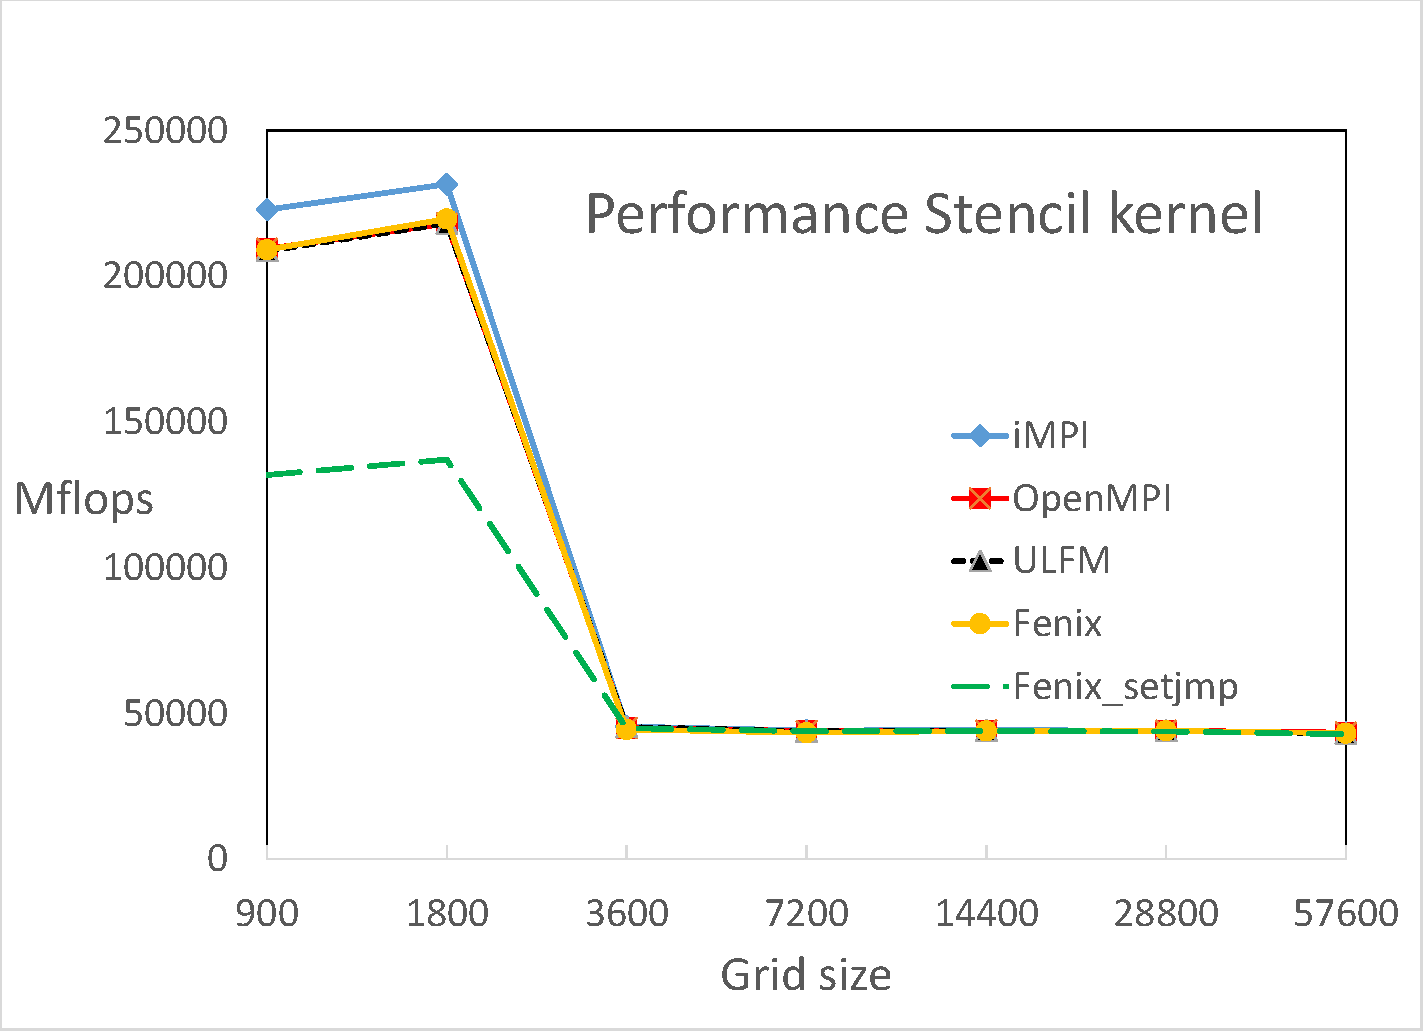
\includegraphics[width=\columnwidth]{stencil_overheads-crop.pdf}
  \caption{Performance of Stencil kernel}
  \label{fig:stencil}
\end{figure}

We repeat the experiment for the Synch\_p2p kernel, see Figure \ref{fig:p2p}.
Most notable is the fact that even for the finest grid of $900^2$ points,
overhead of Fenix relative to OpenMPI and ULFM, is negligible.
In this case we note that the \texttt{setjmp} fix does not make that much
difference.
The reason is that the loop carried dependence in the time consuming part of
the kernel prohibits many compiler optimizations, including vectorization.
We also note the striking differences between the shapes of the performance
curves for Stencil and Synch\_p2p.
For the very fine-grain Synch\_p2p, communications dominate, except for the largest
grids, so larger grids mean better peformance.
For Stencil the reverse is true. Communication do carry a cost for smaller grids,
but that effect is offset by the fact that the whole grid fits in the L2 cache.
Once the data set spills out of that, the code becomes bandwidth bound and
performance decreases.

\begin{figure}
  \centering
  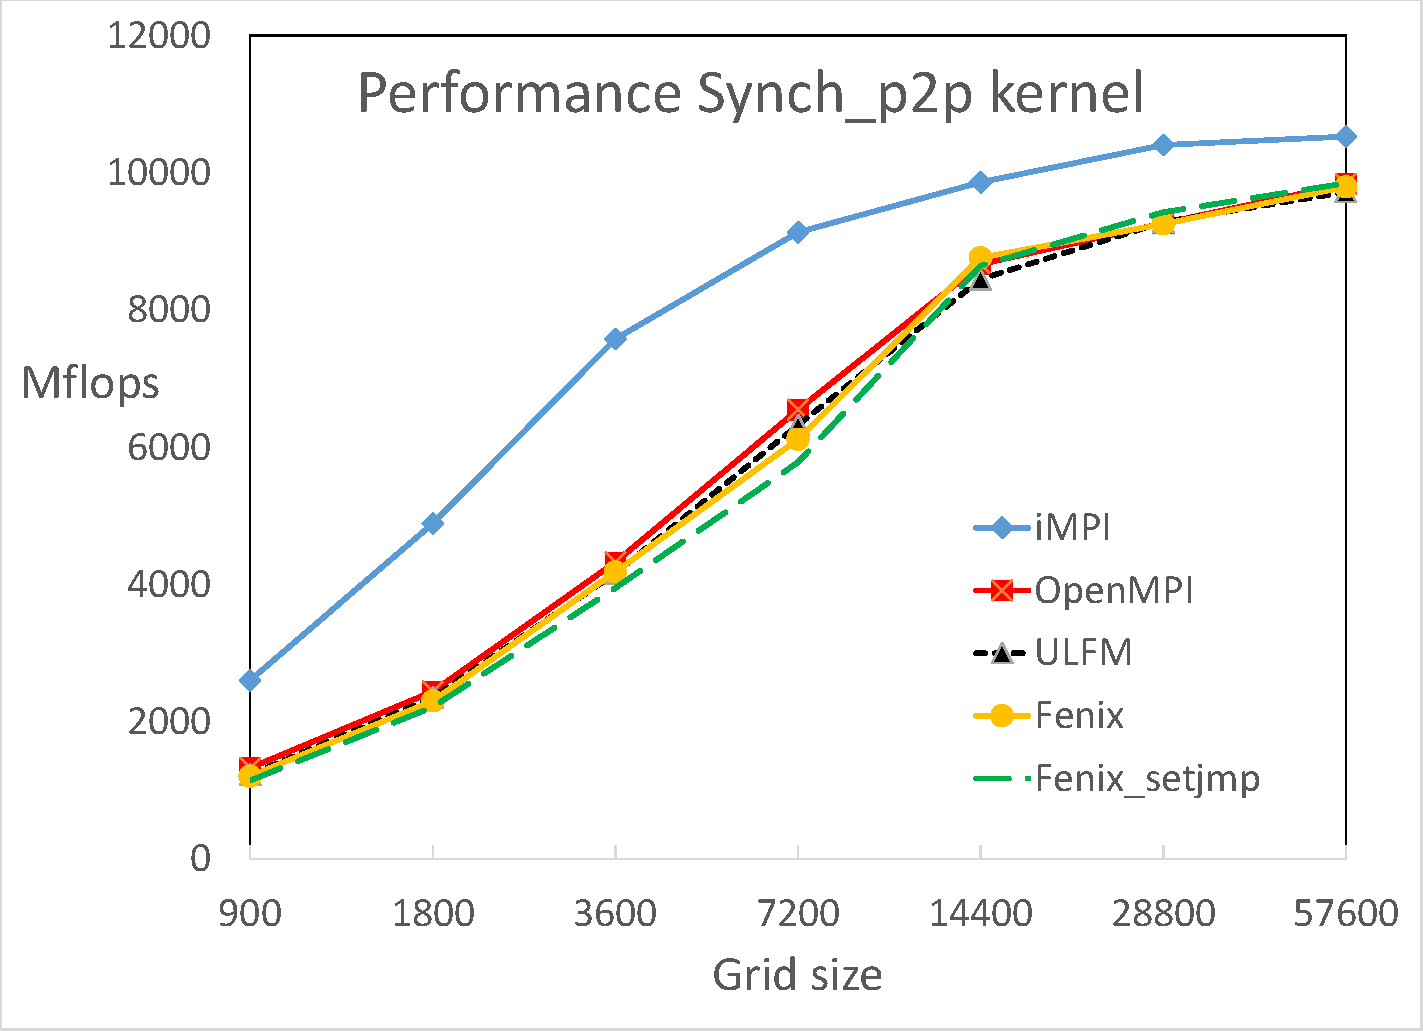
\includegraphics[width=\columnwidth]{p2p_overheads-crop.pdf}
  \caption{Performance of Synch\_p2p kernel}
  \label{fig:p2p}
\end{figure}

The Transpose kernel exhibits an interesting performance difference between
Intel MPI and the OpenMPI-based runtimes for the smallest grids.
At the left (fine-grain) part of the spectrum in Figure \ref{fig:transpose}
it is obvious that the shared memory implementation of the Intel runtime has
been well optimized for an all-to-all communicationb pattern with many small
messages.
This advantage disappears for larger matrices.
However, we again see that there is virtually no noticeable performance
difference between OpenMPI, ULFM, and Fenix, even for very small matrices.

\begin{figure}
  \centering
  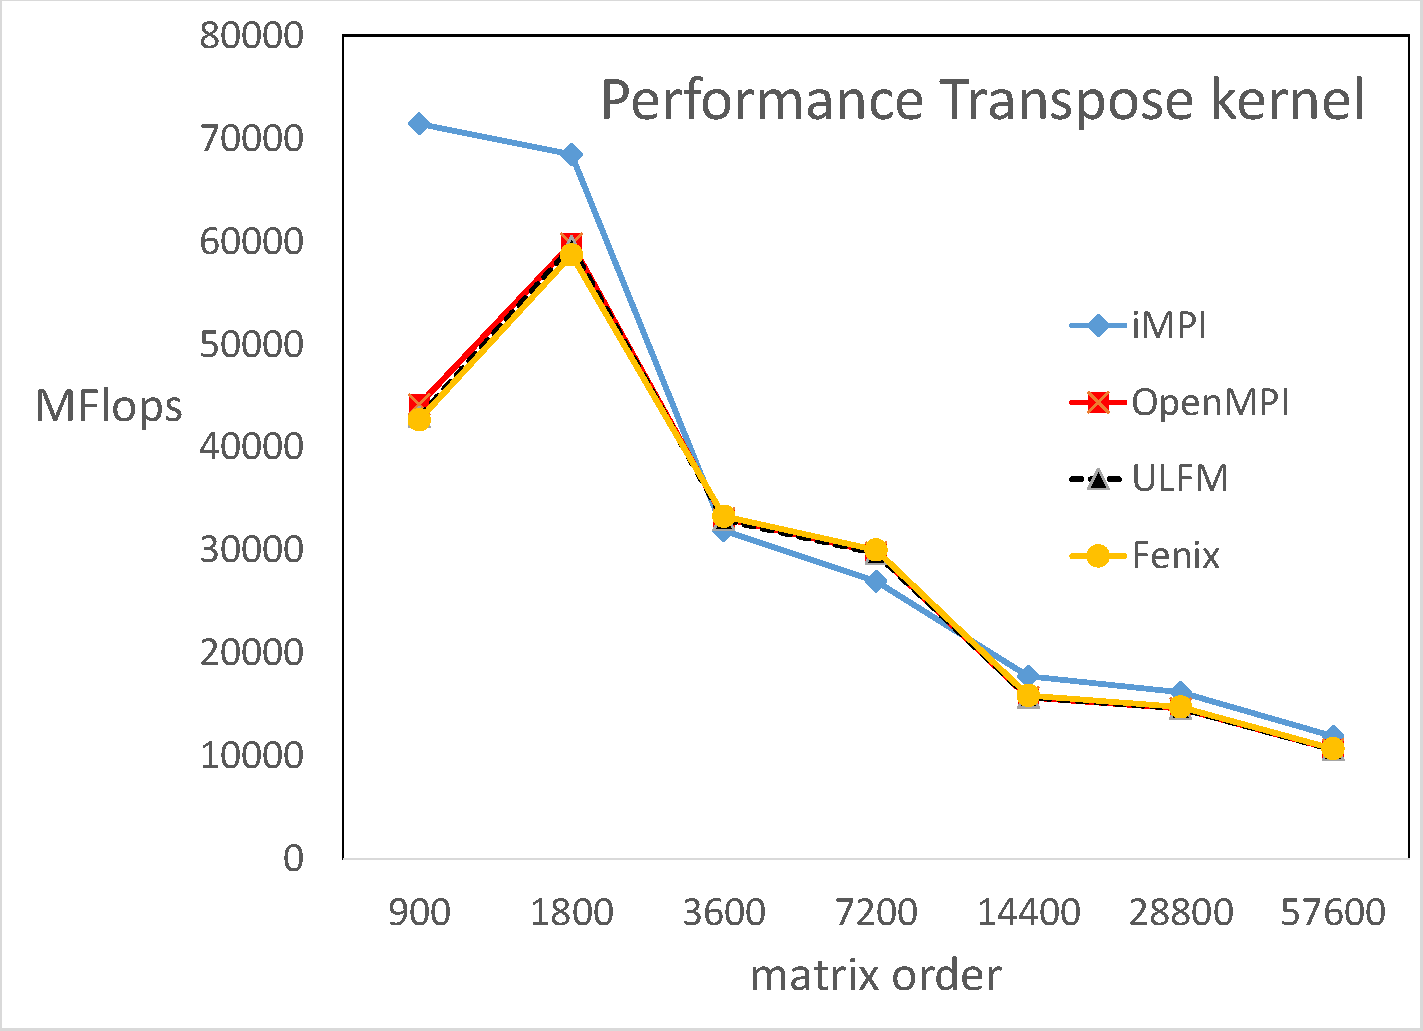
\includegraphics[width=\columnwidth]{transpose_overheads-crop.pdf}
  \caption{Performance of Transpose kernel}
  \label{fig:transpose}
\end{figure}

Finally, in Figure \ref{fig:AMR} we show the results of the AMR kernel.
Again, it is obvious that Fenix and ULFM add negligible overhead to
OpenMPI for this workload.
\begin{figure}
  \centering
  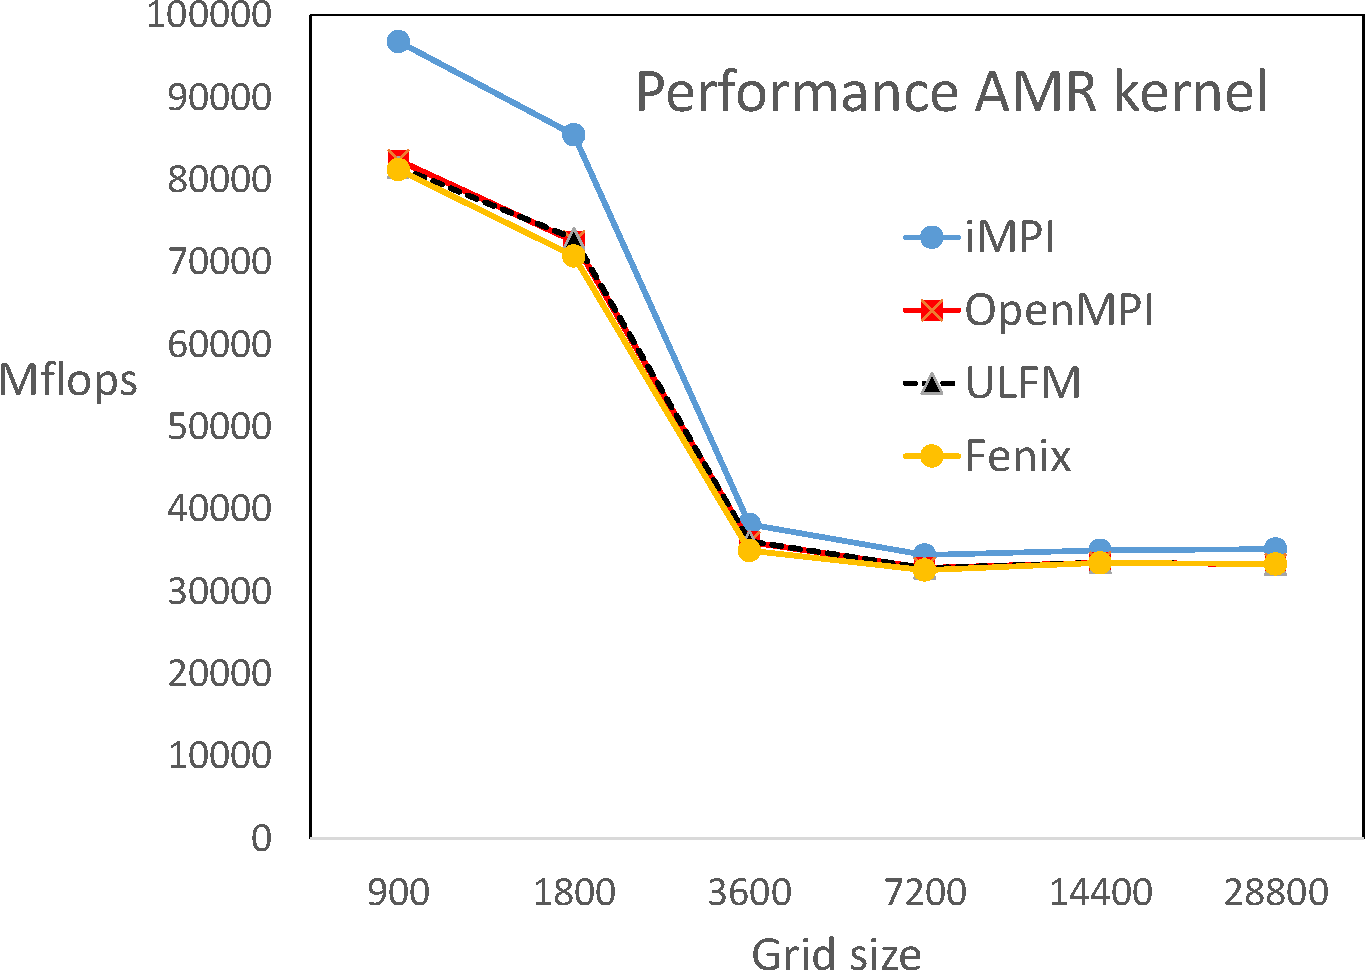
\includegraphics[width=\columnwidth]{AMR_overheads-crop.pdf}
  \caption{Performance of AMR kernel}
  \label{fig:AMR}
\end{figure}
